\documentclass[10pt,twocolumn,letterpaper]{article}

\usepackage{3dv}
\usepackage{times}
\usepackage{epsfig}
\usepackage{graphicx}
\usepackage{float}
\usepackage{amsmath}
\usepackage{amssymb}
\usepackage{subcaption}
\usepackage{lscape}
\usepackage{array}
\usepackage[table]{xcolor} 
\usepackage{numprint}
\usepackage{dsfont} % Ensembles C,R,N ,...
\usepackage{hyperref} % Pour créer des liens hypertexts: \url{my_url}
%Joli tableau 
\usepackage{booktabs}
\newcommand{\ra}[1]{\renewcommand{\arraystretch}{#1}}

% Include other packages here, before hyperref.

% If you comment hyperref and then uncomment it, you should delete
% egpaper.aux before re-running latex.  (Or just hit 'q' on the first latex
% run, let it finish, and you should be clear).
%\usepackage[pagebackref=true,breaklinks=true,letterpaper=true,colorlinks,bookmarks=false]{hyperref}

\threedvfinalcopy % *** Uncomment this line for the final submission

\def\threedvPaperID{007} % *** Enter the 3DV Paper ID here
\def\httilde{\mbox{\tt\raisebox{-.5ex}{\symbol{126}}}}

% Pages are numbered in submission mode, and unnumbered in camera-ready
\ifthreedvfinal\pagestyle{empty}\fi
\setcounter{page}{1}
\begin{document}

%%%%%%%%% TITLE
\title{Beehive Traffic}

\author{Students:\\
Julie Veya\\
Jonathan Burkhard\\
Jasmin Fischli\\
Philipp Goldlin\\
{}
% For a paper whose authors are all at the same institution,
% omit the following lines up until the closing ``}''.
% Additional authors and addresses can be added with ``\and'',
% just like the second author.
% To save space, use either the email address or home page, not both
\and
Supervisor:\\
Dr. Torsten Sattler\\
\\
{}
}

\maketitle
%\thispagestyle{empty}

%%%%%%%%% ABSTRACT

\begin{abstract}

   Honey is a precious good and thus beekeepers want to protect their harvest. In spring, bees may be swarming to find a better place to live, so beekeepers can lose some colonies. With the help of computer vision tools, we implemented two different algorithms to detect this phenomenon. We used a GoPro setup to collect videos of the entrance of one of our colleague's hive. The algorithms are based on a background subtraction to find the moving objects. We then applied a filter by histogram comparison to find out whether a moving object is a bee or not. We then saved the position of each bee which allowed us to track them and finally count the incoming and outgoing flow of bees.
   
\end{abstract}

%%%%%%%%% BODY TEXT

\section{Introduction}

From the beginning of time, animals and humans have always been searching for better places to live, and the same applies for bee colonies. They swarm because of various reasons, for example, the queen may be too old or the weather conditions may not be good enough. In the first two days, they move near the hive and send some bees to search for a favorable location, which can sometimes be far away. Once they found it, they will settle there. A swarming is a massive event, where a big part of the colony can suddenly fly away. The issue for a beekeeper is to regularly check on his hives in order to prevent the loss of a colony and with it the honey to harvest. \\
To help beekeepers catch the colonies which have swarmed and enable them to know when this happens, we suggested to count the incoming and outgoing flow of bees with computer vision tools. As a swarming consists in a peak of outgoing activity, the idea is to be able to detect these peaks and thus alert the beekeeper in such cases. The algorithms we created are written in Python and based on OpenCV libraries. They are based on background subtraction to recognize the objects in motion and the use of filters and histogram comparison to determine whether such objects are bees or not. Secondly, the bee positions are stored, allowing us to track and count the incoming and outgoing flow of bees. 

%-------------------------------------------------------------------------

\subsection{Related work}

So far, beekeepers did not use any tools to detect swarming. But with the progress of technology, there are more and more possible processes to fulfill this purpose.\\
A simpler method to detect swarming is to measure the sound close to the hive entrance. Through the noise created by the bees, a colony's swarming can then be detected \cite{Authors_Papper_1}. Another way to recognize swarming is to measure the temperature inside the hive. Indeed, around 10 to 20 minutes before a spread, the temperature increases from $34-35^\circ C$ to $37-38^\circ C$ \cite{Authors_Papper_2}. This requires a very accurate temperature sensor, placed near the bee cluster. Given that the cluster steadily changes its location inside the hive, it is hard to obtain reliable information from this method.\\
Some people use computer vision to detect and track animal movements. For example, the University of Washington in St-Louis created an algorithm on C++ to track ants \cite{Authors_BioTracking}. On YouTube, there are a lot of videos showing the results of different computer vision algorithms, where we can see some good tracking implementations \cite{Authors_Youtube_1} \cite{Authors_Youtube_2}  \cite{Authors_Youtube_3}. Unfortunately, they do not explain how they reached those results, but in \cite{Authors_Youtube_1} and \cite{Authors_Youtube_2} bees are moving very slowly, which implies an ease to track them.


%------------------------------------------------------------------------
\section{Task distribution}
In a first phase, all team members were getting familiar with Python and OpenCV and doing literature research. By this, we obtained a broad basis of ideas and concepts for the development of our algorithms. Soon we decided for two main algorithms to be pursued. \\
Jasmin and Philipp were mainly in charge of implementing codes of the ideas which had been discussed in the group and trying out various parameters and methods for improving the results.
Jonathan was in charge of the setup at the hive and of taking videos of the bees in various weather conditions and camera settings. Moreover he took care of Latex-formatting, gitHub organization and establishing order in the written codes to keep them clean. \\
Julie was keeping a general overview of the development and counseling by doing further literature research. Moreover she took the main responsibility for the presentations and the final report. 
The writing of content in the presentations, poster and report was equally distributed among all the team members.

%------------------------------------------------------------------------

\section{Experimental setup}

To reach our goals for this project, we used a GoPro Hero3, a support for the camera designed and 3D printed by us, a bee colony and one hive.

To reproduce the video, we placed the camera on the support which is fixed on the roof above the board of flight. This allowed us to have the whole entrance area and all the bees around it in every scene.

\begin{figure}[h!]
\centering
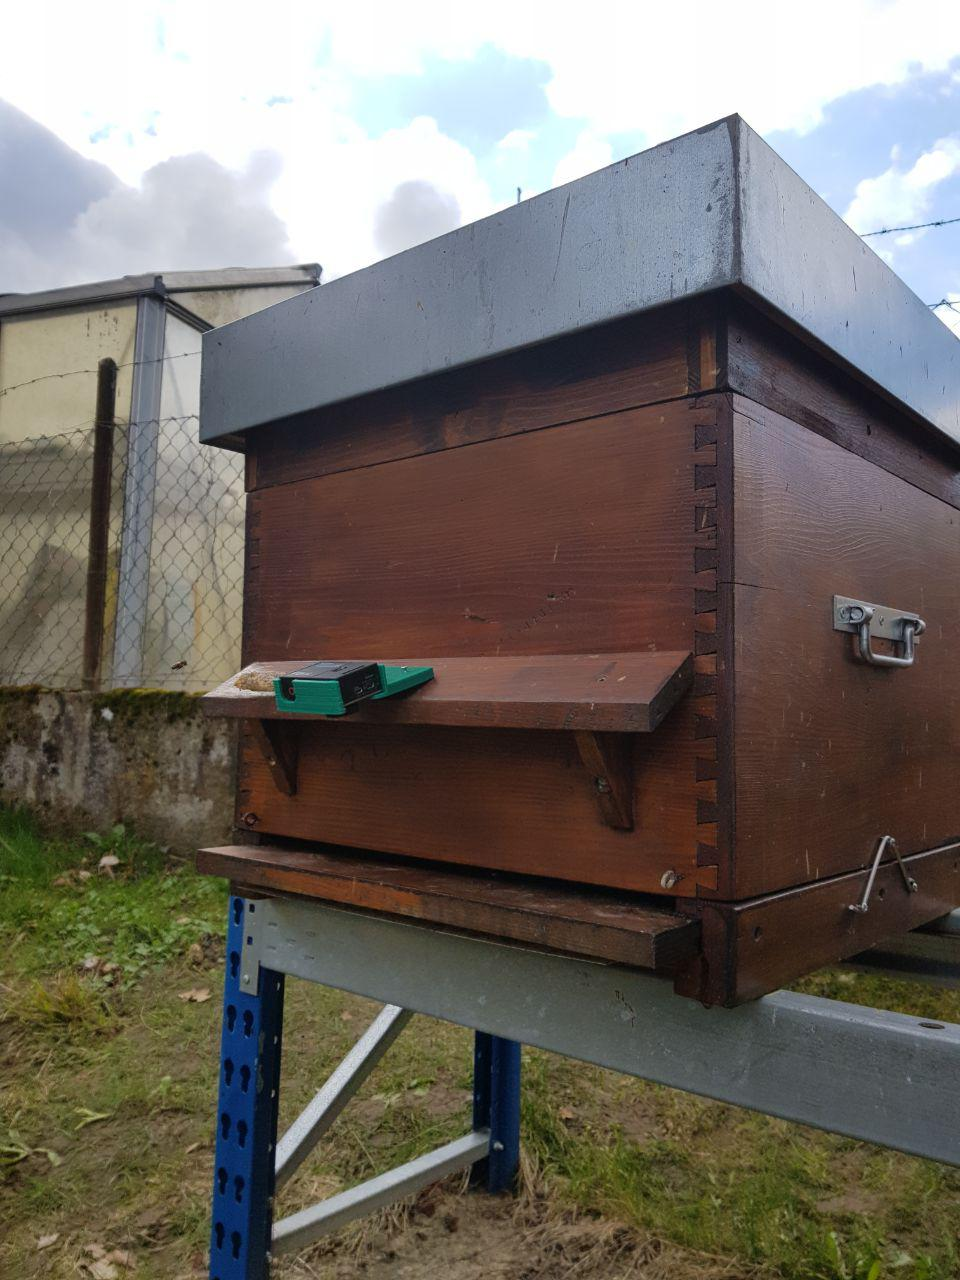
\includegraphics[scale=0.23]{pictures/photoSupport.jpg}
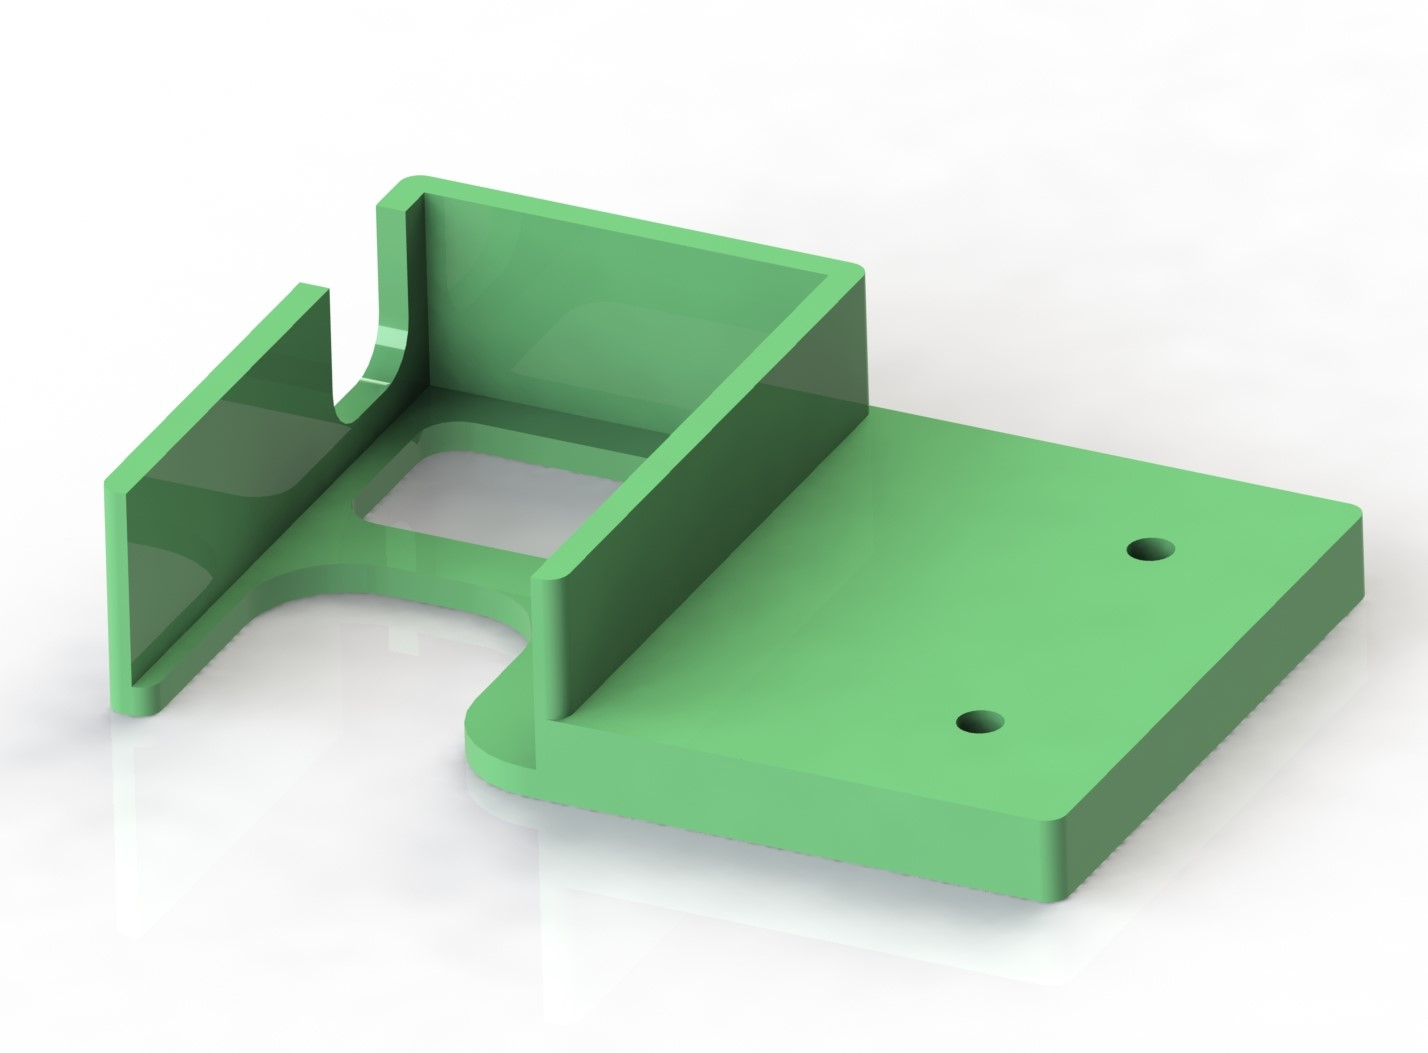
\includegraphics[scale=0.1]{pictures/support.jpg}
\caption{Support and mounting of the GoPro}
\end{figure}

Due to the wide angle of the GoPro, there is a lot of distortion in the image. So we first calibrated the camera in order to rectify the images.
 
The library of OpenCV \cite{Authors_OpenCV} is used to calibrate the camera. First, we used a black and white pattern in front of the camera at different localisations in order to measure the deformation. With these images, we generated a matrix which remaps the distorted image.

\begin{figure}[h!]
\centering
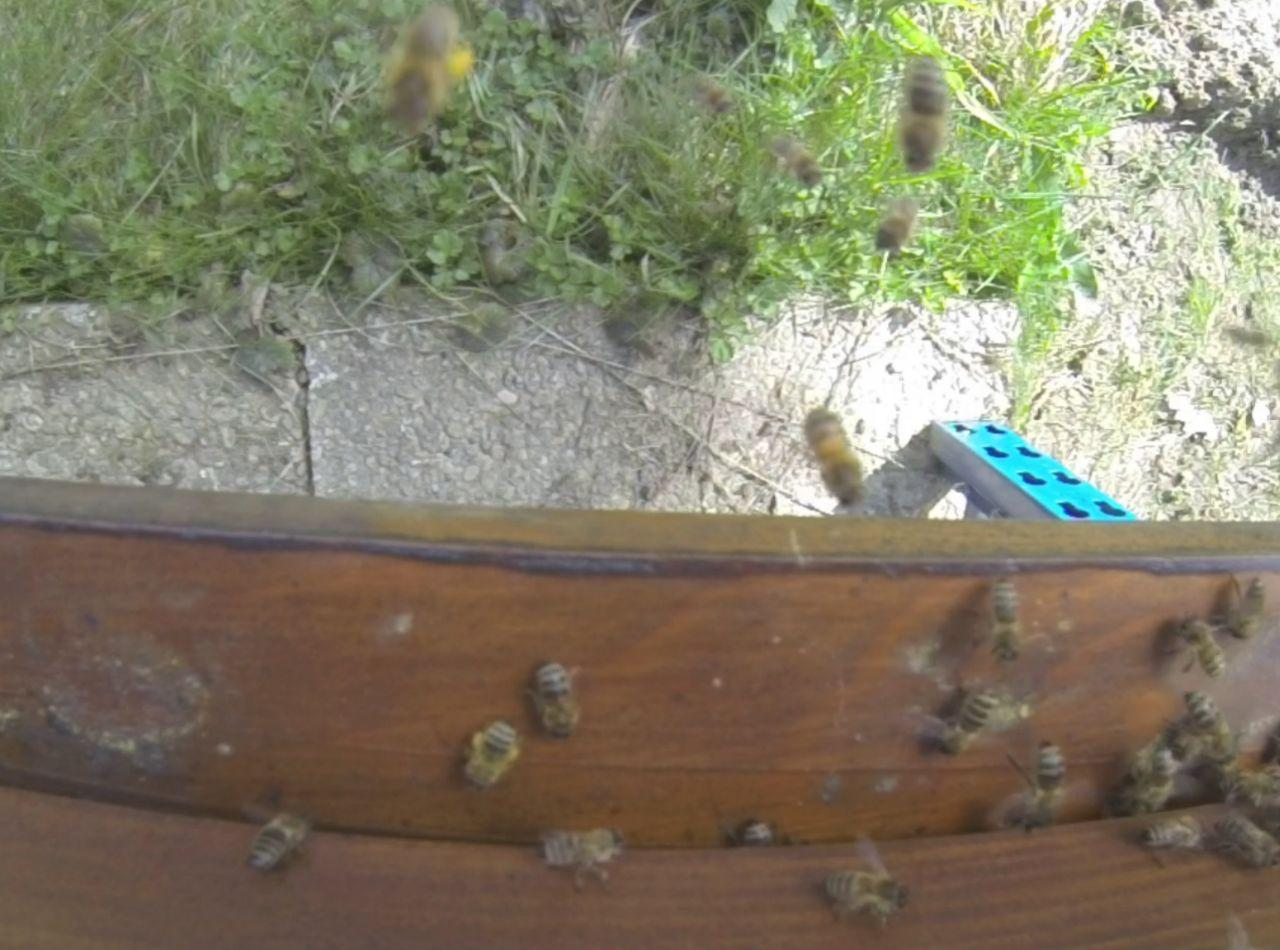
\includegraphics[scale=0.22]{pictures/Dist.jpg}
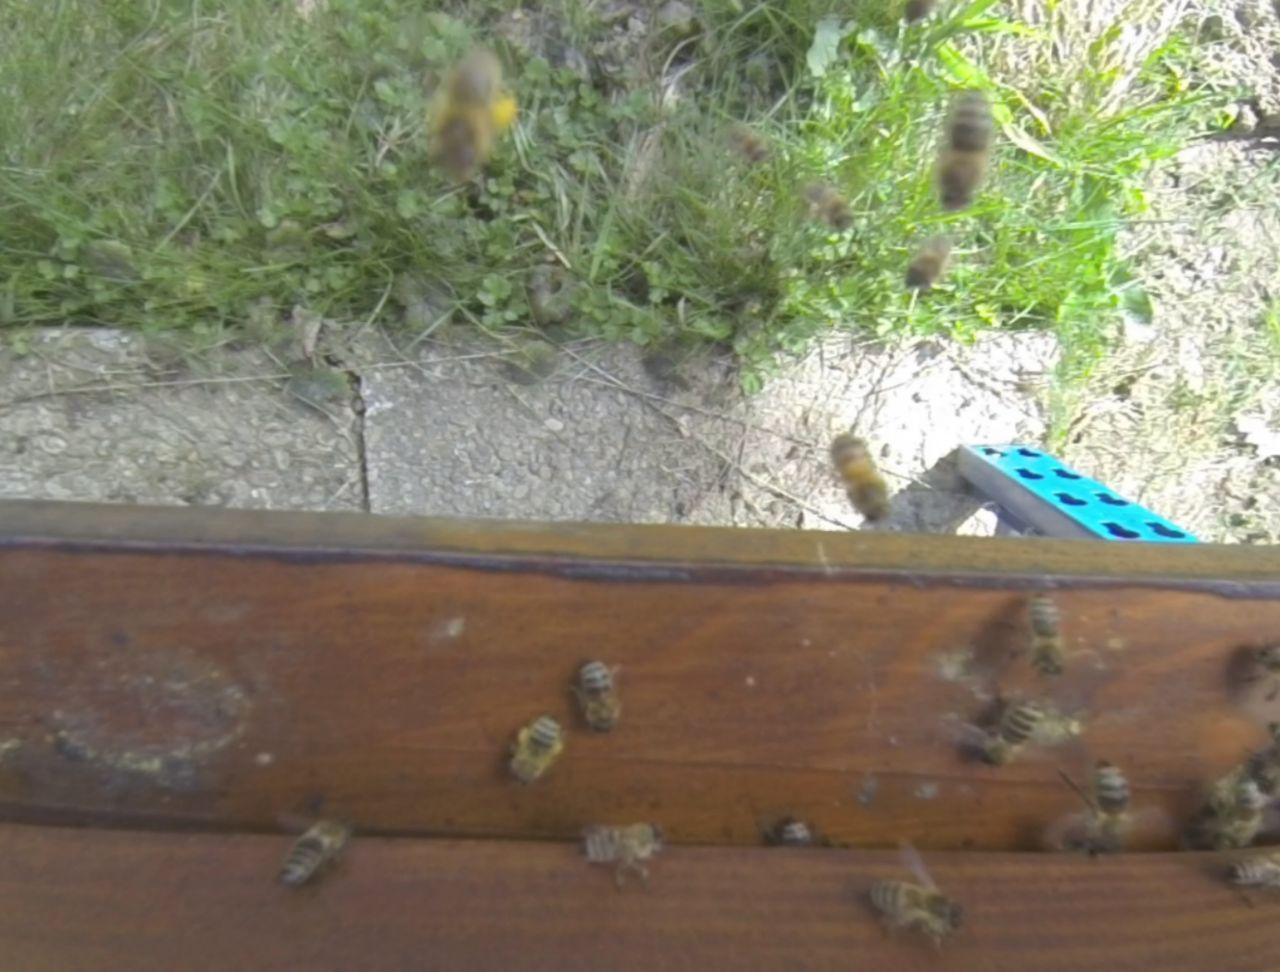
\includegraphics[scale=0.22]{pictures/Calib.jpg}
\caption{Original distorted image (left) and rectified image (right)}
\end{figure}

However, for the sake of simplicity we defined a straight line, 5 cm in front of the actual hive entrance for counting the bees. We did it this way, because right next to the entrance, there are often bees sitting in groups or moving slowly. As a result, the detection is prone to errors in this area. By simply defining bees above the blue virtual entrance line (see Fig. 3) to be outside and the ones below the line to be inside the hive, we made counting easier, without significantly changing the net result. Moreover, this simplification allowed us to use our algorithms without any calibration and thus save computation time.

\begin{figure}[h!]
\centering
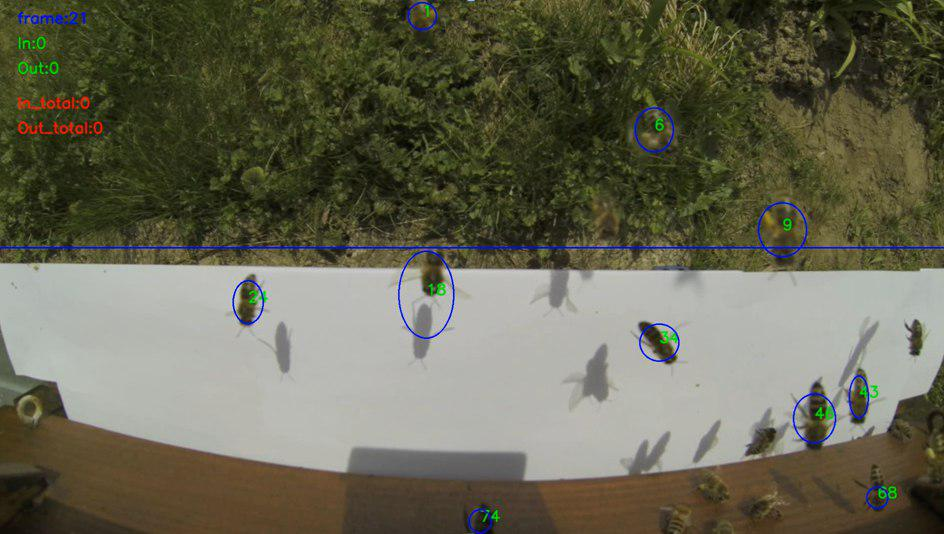
\includegraphics[scale=0.26]{pictures/ph.jpg}
\caption{A white paper is placed on the board of flight to improve the recognition of the bees}
\end{figure}

%-------------------------------------------------------------------------
\section{First algorithm}
This algorithm uses background subtraction for the detection of the bees.
To reduce false recognition of bees, we first apply different filters, such as a threshold and a median filter, before continuing the detection. This already reduces a big part of the error source. After the filters, the algorithm looks for all the present contours and stores them in an array. For each contour, we control whether the area is big enough. If so, it is probable that the contour contains a bee.\\
The algorithm creates a list of objects with all the present bees. An object of the class \textit{Bee} contains information about the bee, such as the position, the speed and the status of the bee. The status tells us if the bee has been lost during the last couple of frames and if so, it allows us to count for how many frames it has been lost.\\
In each frame, a new list with bees is created. In a next step, the algorithm calculates the distance between the position of the bees from the old frame and the bees from the current frame. This step is different to the second algorithm. Instead of comparing the distance of the positions between all the new bees and all the old bees, the algorithm just takes the position of the first old bee from the table and compares it with all the new bees and then matches it to the closest one, which is still within a certain distance to the bee and removes the corresponding bee from the array with the new bees. The algorithm continues until there are no more old bees left. If a bee is lost, the algorithm counts for how many frames the bee was lost, and with each increasing frames, it looks in a larger region for the bee. If the bee is lost for too long, the algorithm ignores this bee for the rest of the video.\\
For the remaining bees in the new array, the algorithm checks if it is possible that they entered the frame in this instance and if the bee is within this region, it adds the newly entered bee into the list containing all the bees. As a result, it is not necessary to check the histogram of the bees, because the area where the histogram check is important, is in the middle of the image on the white background. Therefore the first algorithm is a lot faster than the second.


\section{Second algorithm}

This algorithm consists of three main parts: the bee recognition, the matching of bees in consecutive frames and the counting of the bee flow. As for the first algorithm background subtraction builds the basis of our bee recognition. This allows for segmentation of moving and static parts of the image. To filter out noise, we apply a median filter and a combination of erosion and dilation. In the resulting binary image, we label each moving patch with a number by using connected components. There might be moving parts in the scene, other than bees. Therefore, we use an area threshold in order to sort out smaller patches which are unlikely to belong to a bee. What remains, are the moving bees and their shadows, which are mainly visible in the white entrance area. To distinguish the shadow from bees, we created an average color histogram of numerous bees and shadows from several videos. By using a scalar product, we compare them to the actual histograms of the moving objects and thereby decide whether it is a shadow or a bee.\\
In order to find out whether a bee is entering or leaving, the key is to be able to match the corresponding bees of the current frame with the ones of the previous frame. This task is not always easy, as bees often move in an unpredictable way and frequently overlap with each other. We found that a good result can be generated by creating a matrix containing distances between all the bees of the last frame with all the bees of the current frame. The algorithm then first searches for the overall minimum distance and connects the two corresponding bees. This step is repeated with the remaining bees until a certain distance threshold is reached. The remaining ones are not matched as it is unlikely to be a distance travelled by a bee during the time between two frames. This often occurs when bees are entering or leaving the scene.\\

Around the entrance slot of the hive, bees are often sitting for a long time or moving slowly, which complicates their recognition. We avoid this problem by defining rectangular box around the entrance slot. This results in simply having the two distinct regions, inside and outside. Thus, every bee that enters this box is considered to have entered the hive and vice versa and the corresponding counters are incremented.

\section{Results}

We tested our algorithms on four different videos. For each video, we took the first 400 frames and counted the incoming and outgoing bees  with our algorithms ($in_{counter}$ and $out_{counter}$) as well as manually ($in_{manual}$ and $out_{manual}$). We did this for each video in sequences of 50 frames and then compared the obtained numbers. We then computed the relative error for each sequence, $\eta_{in} =|\frac{in_{manual} - in_{counter}}{in_{manual}}|$ and $\eta_{ηout} = |\frac{out_{manual} - out_{counter}}{ out_{manual}}|$, as well as their mean relative error over all the sequences, $\eta_{in}^{mean}$ and $\eta_{out}^{mean}$. 
%The spreadsheet is given in the annex as well as the graphs corresponding to these results. 
%We show below the graphs for the video that gave us the best result, i.e video \textit{1355FPS60}.
%For the video displayed, video \textit{1355FPS60}, we obtained the following mean relative errors :

%\begin{table} [h!]
%\centering
%\captionof{table}{Mean relative errors} \label{tab:title} 
%\ra{1.3}
%\begin{tabular}{@{}lll@{}}\toprule
%  & Algorithm 1 & Algorithm 2 \\ 
%\midrule
%$\eta_{in}^{mean}$ &  0,664732143 & 0,472916667 \\
%$\eta_{out}^{mean}$ & 0,311458333 & 0,335416667  \\
%\bottomrule
%\end{tabular}
%\end{table}

\clearpage
\begin{figure}[H]
\centering
\begin{subfigure}[b]{0.35\textwidth}
        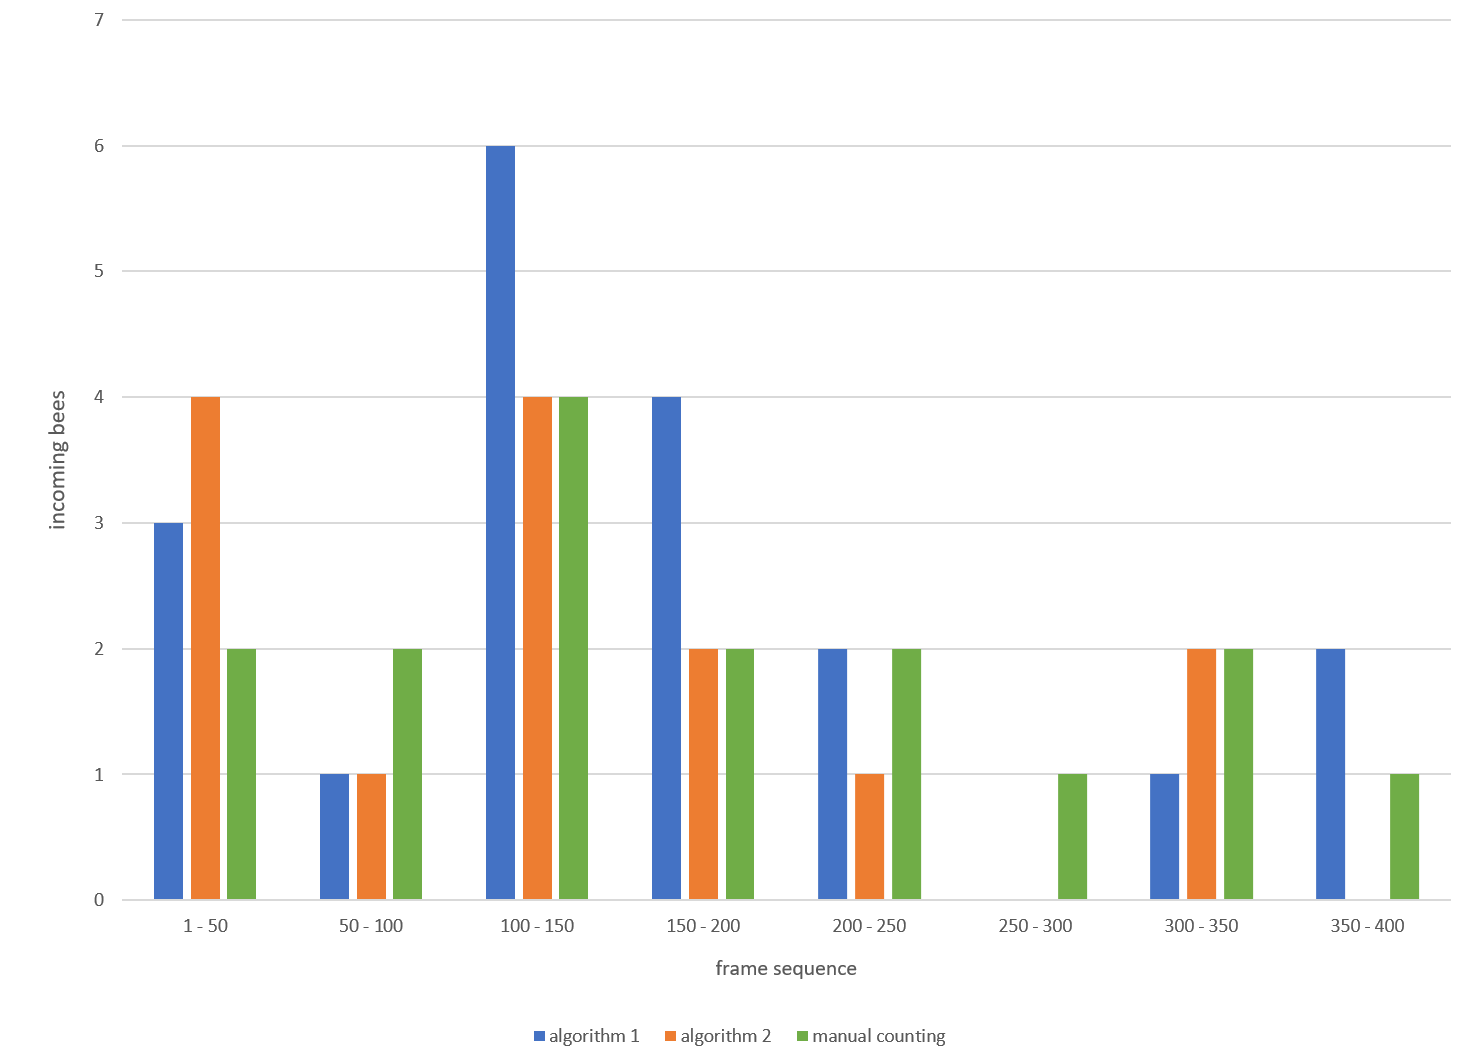
\includegraphics[width=\textwidth]{graphs/video1_incoming_number_of_bees}
        \caption{incoming number of bees}
        \label{fig:vdo1i}
    \end{subfigure}
    \begin{subfigure}[b]{0.35\textwidth}
        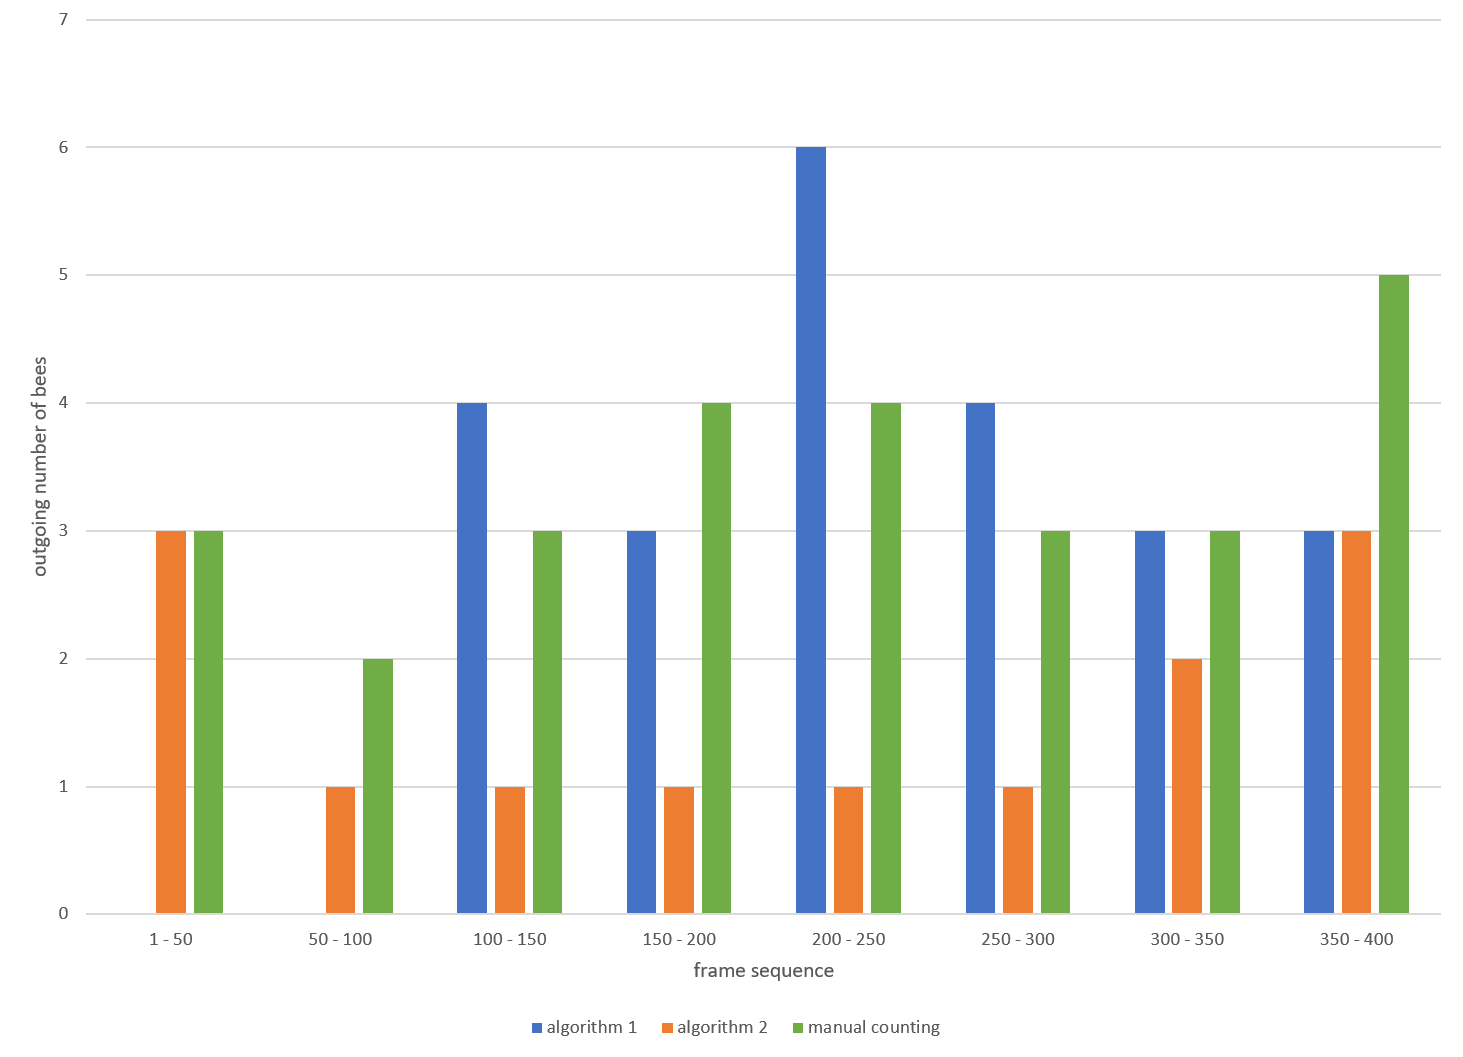
\includegraphics[width=\textwidth]{graphs/video1_outgoing_number_of_bees}
        \caption{Outgoing number of bees}
        \label{fig:vdo1o}
    \end{subfigure}
\caption{counting performance for video 1}
\label{fig:????}
\end{figure}
\begin{figure}[H]
\centering
    \begin{subfigure}[b]{0.35\textwidth}
        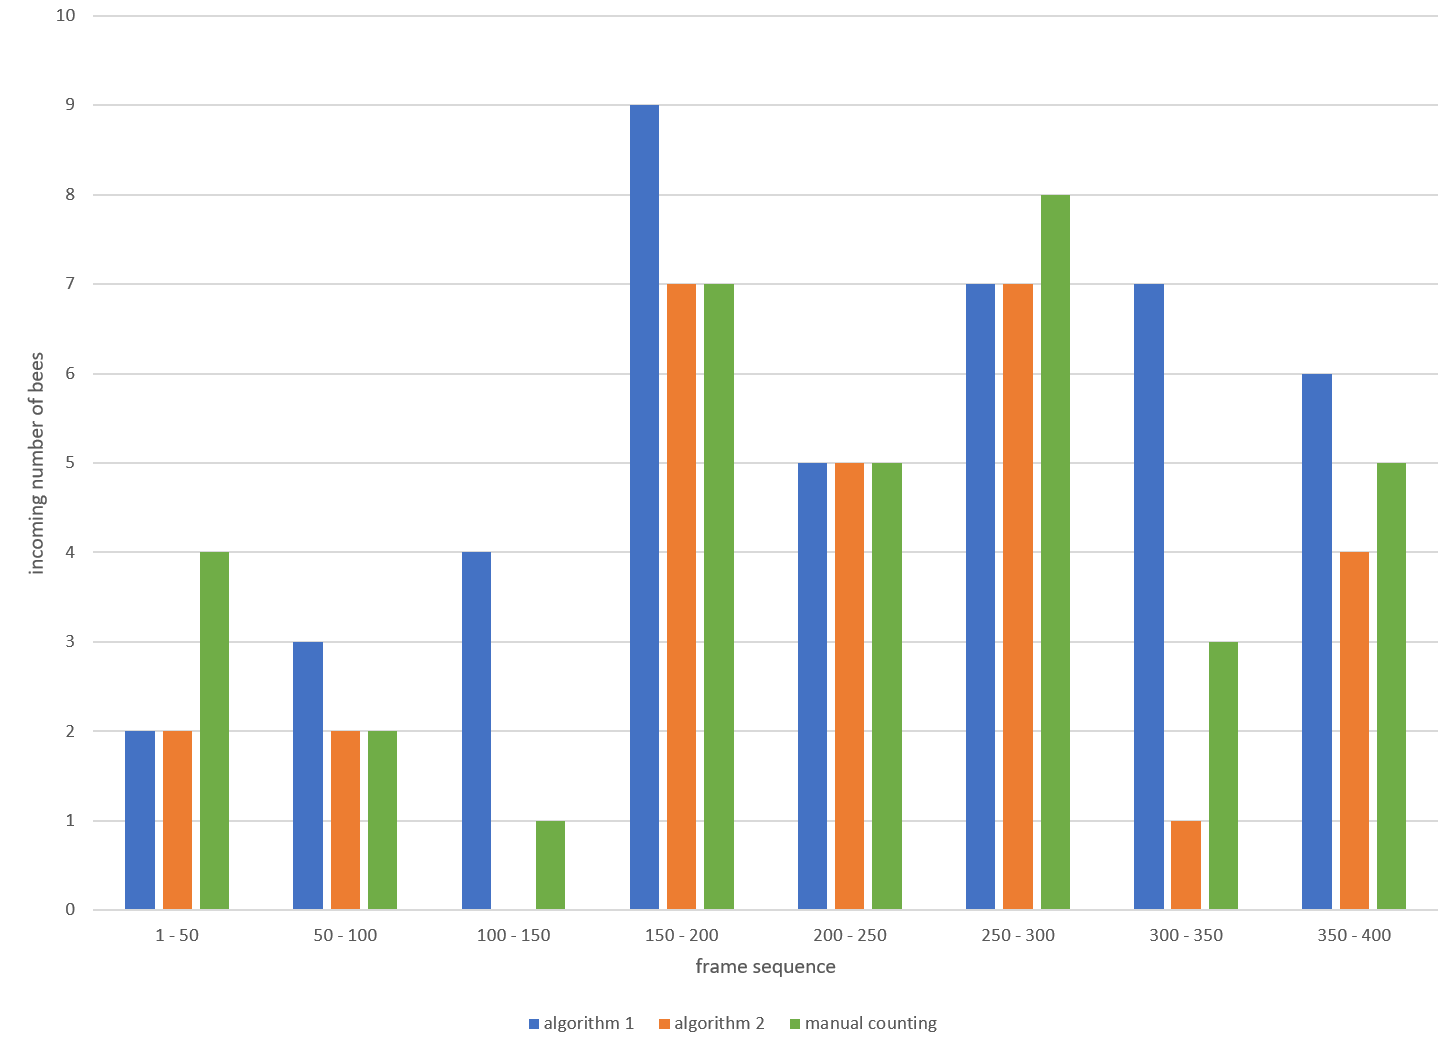
\includegraphics[width=\textwidth]{graphs/video2_incoming_number_of_bees}
        \caption{incoming number of bees}
        \label{fig:vdo2i}
    \end{subfigure}
    \begin{subfigure}[b]{0.35\textwidth}
        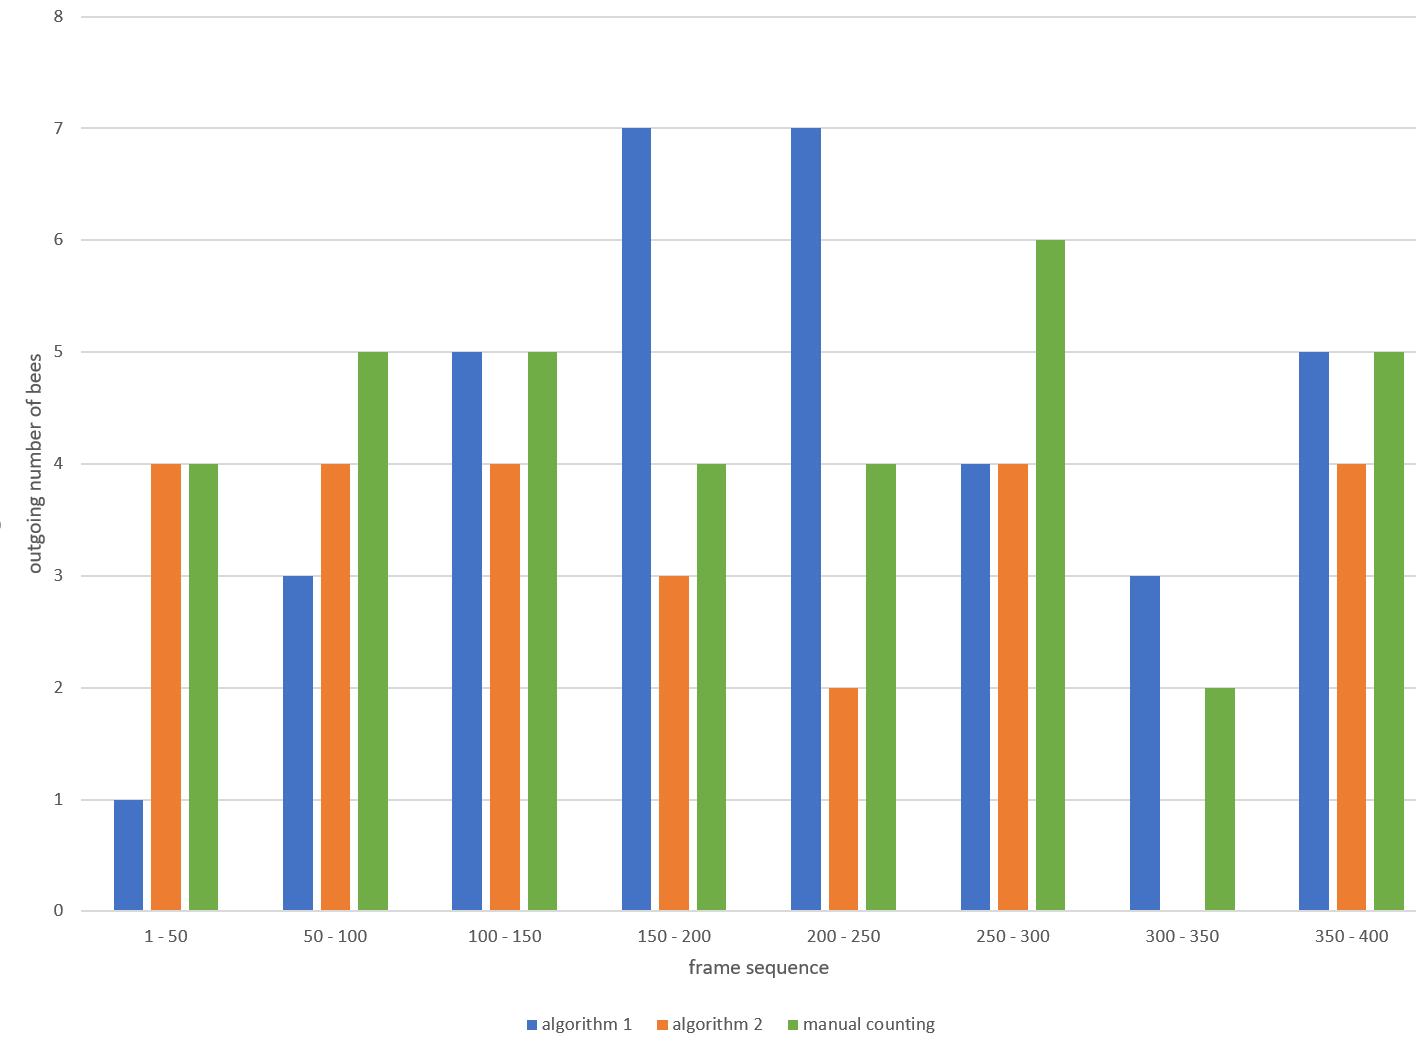
\includegraphics[width=\textwidth]{graphs/video2_outgoing_number_of_bees}
        \caption{Outgoing number of bees}
        \label{fig:vdo2o}
    \end{subfigure}
\caption{counting performance for video 2}
\label{fig:????}
\end{figure}
\begin{figure}[H]
\centering
    \begin{subfigure}[b]{0.35\textwidth}
        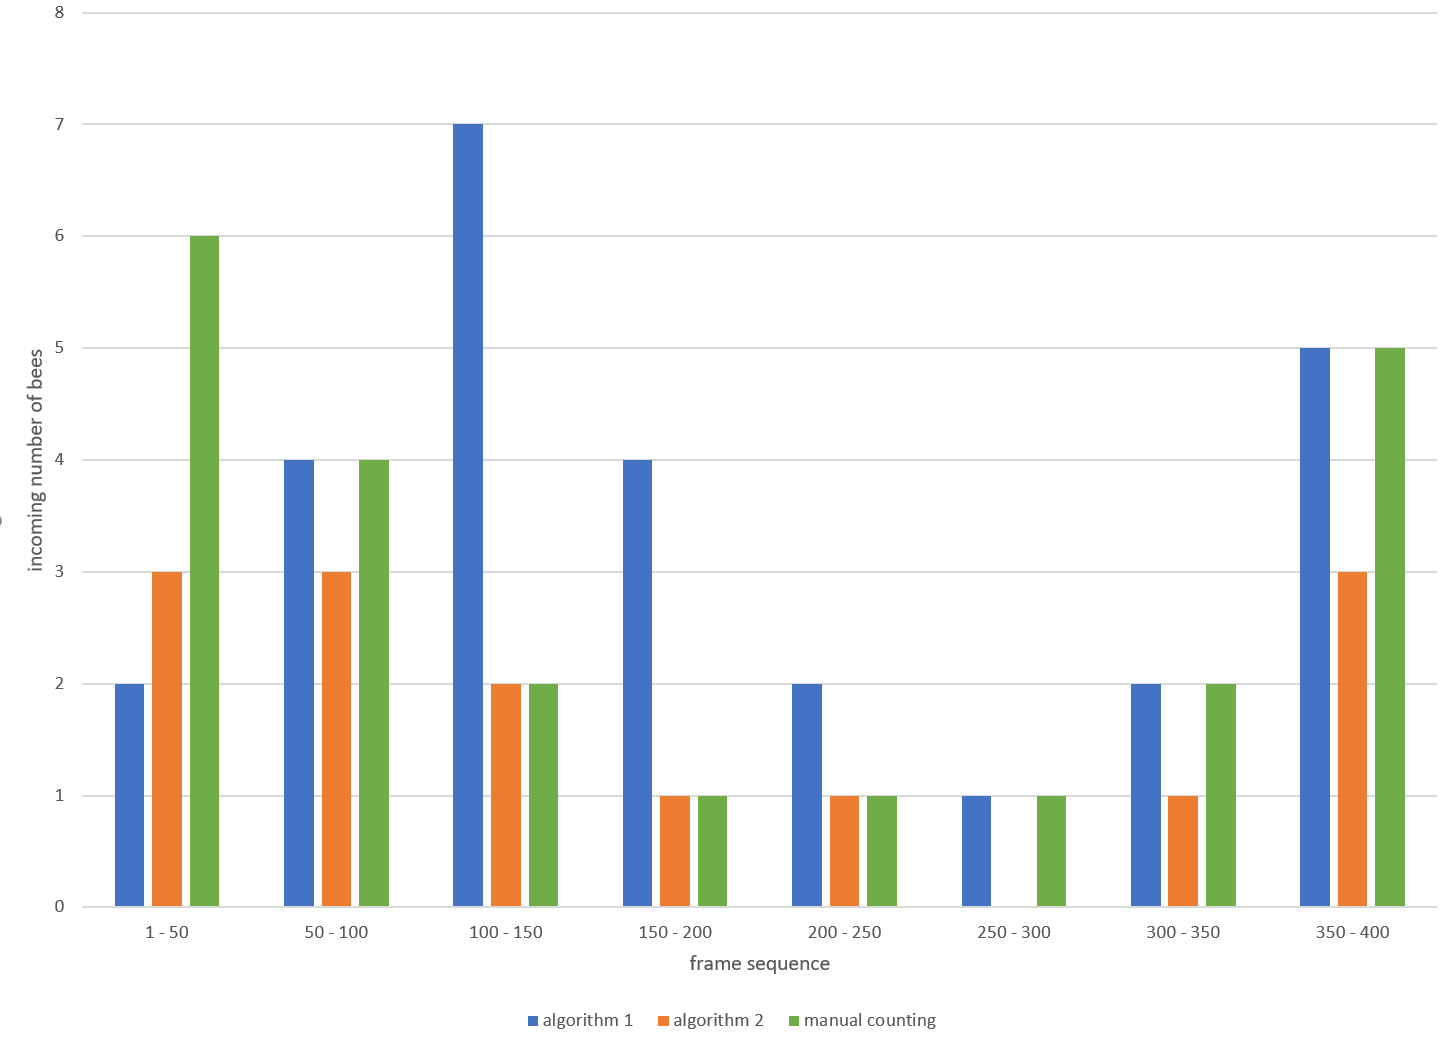
\includegraphics[width=\textwidth]{graphs/video3_incoming_number_of_bees}
        \caption{incoming number of bees}
        \label{fig:vdo3i}
    \end{subfigure}
    \begin{subfigure}[b]{0.35\textwidth}
        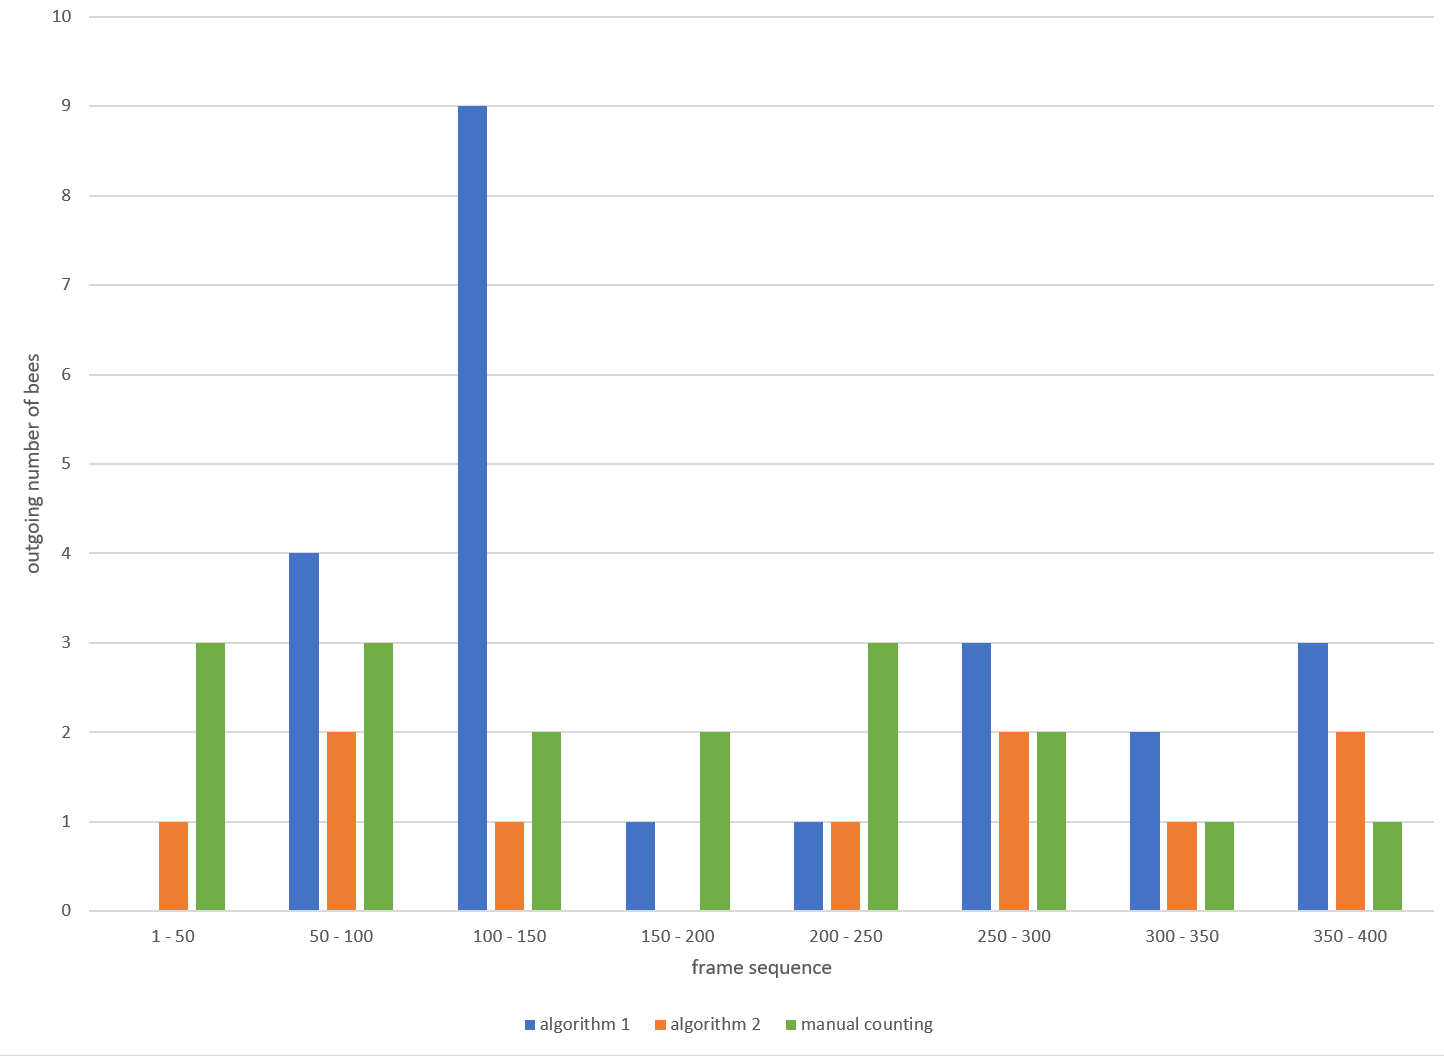
\includegraphics[width=\textwidth]{graphs/video3_outgoing_number_of_bees}
        \caption{Outgoing number of bees}
        \label{fig:vdo3o}
    \end{subfigure}
    \caption{counting performance for video 3}
\label{fig:????}
\end{figure}
\begin{figure}[H]
\centering
    \begin{subfigure}[b]{0.35\textwidth}
        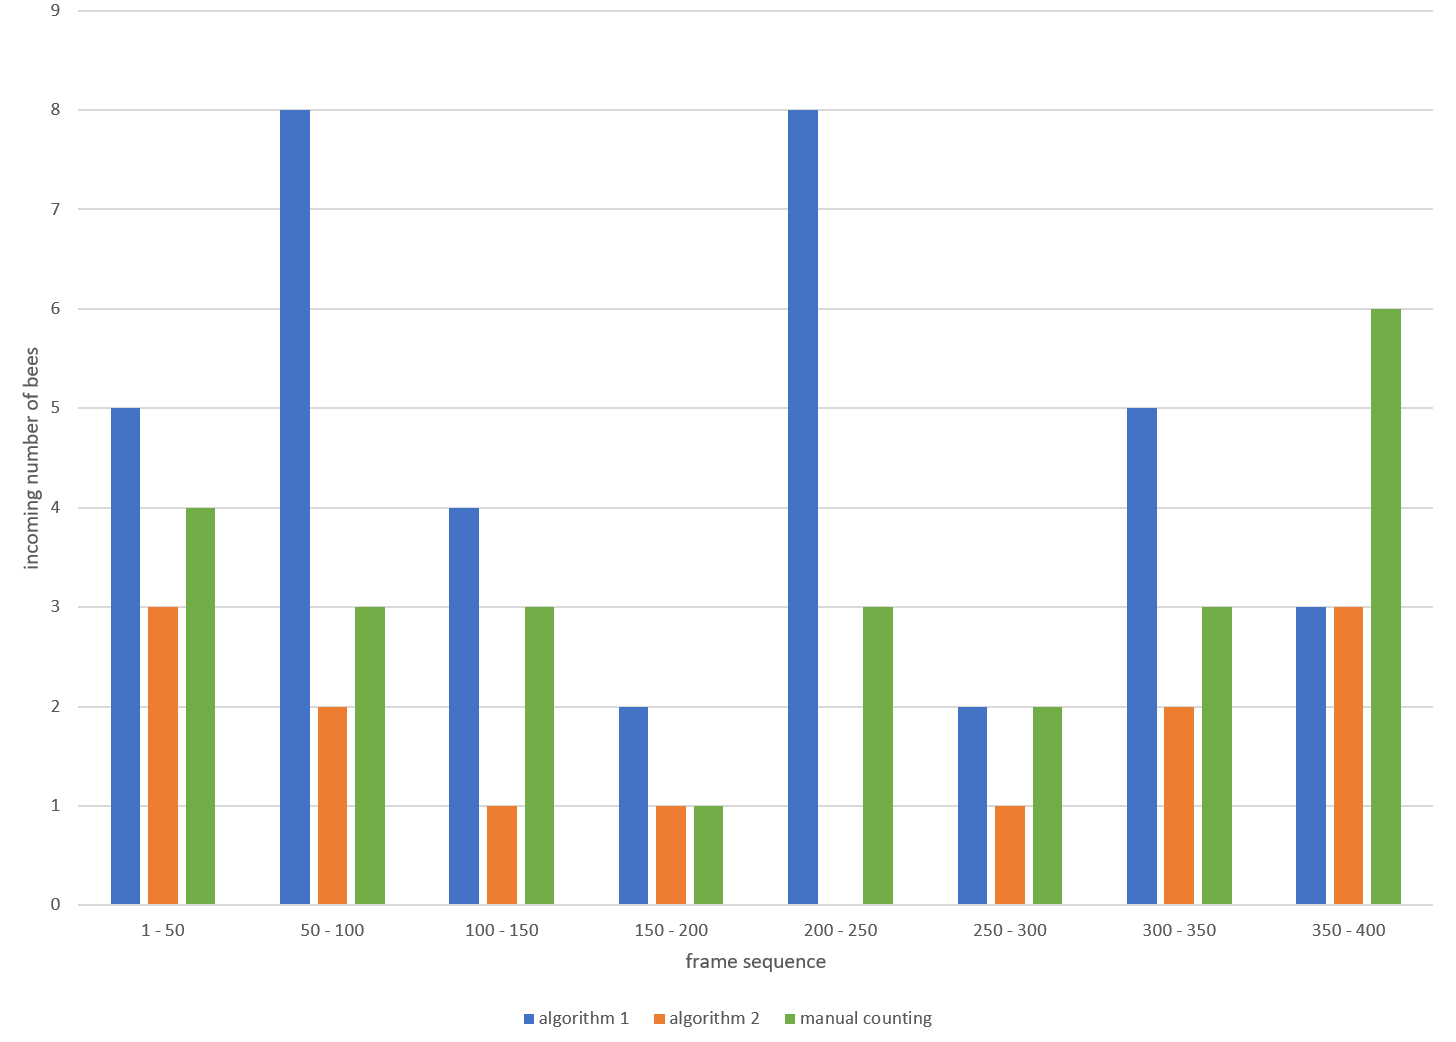
\includegraphics[width=\textwidth]{graphs/video4_incoming_number_of_bees}
        \caption{incoming number of bees}
        \label{fig:vdo4i}
    \end{subfigure}
    \begin{subfigure}[b]{0.35\textwidth}
        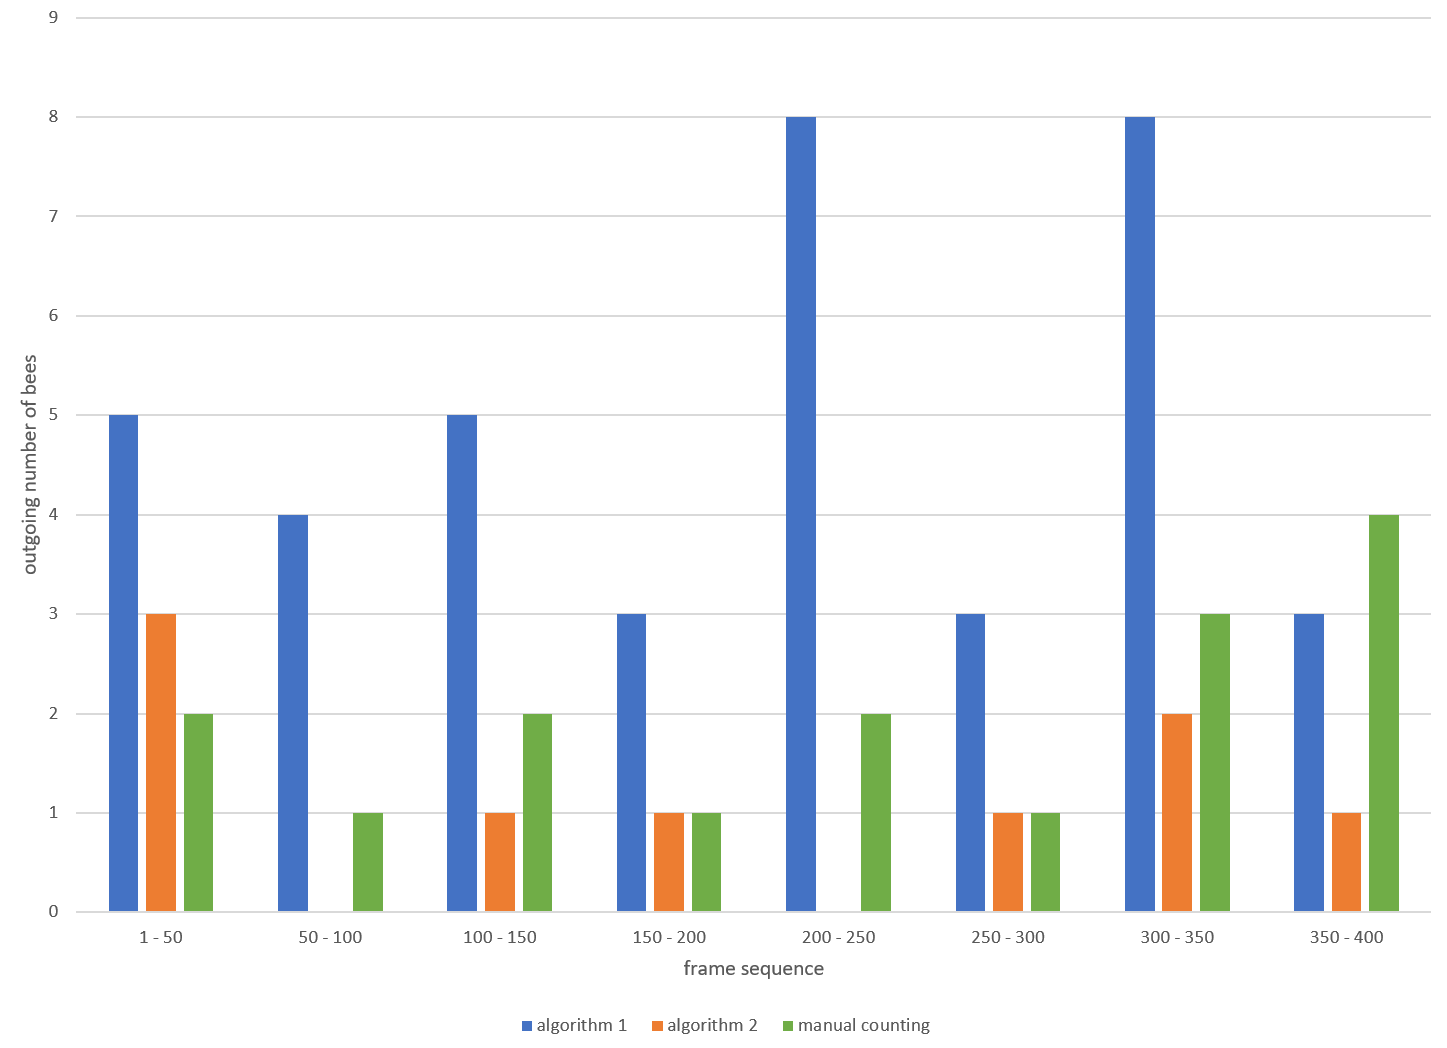
\includegraphics[width=\textwidth]{graphs/video4_outgoing_number_of_bees}
        \caption{Outgoing number of bees}
        \label{fig:vdo4o}
    \end{subfigure}
\caption{counting performance for video 4}
\label{fig:????}
\end{figure}

\section{Discussion}

As the graphs show, in general, the first algorithm counts more bees than the second algorithm. We also see that algorithm 2 gave most of the time better results in terms of the mean relative error. In some sequences, both algorithms perform really well and on others they perform quite poorly. We also see for algorithm 2, that the error is smaller for video 2 and 3 than for video 1 and 4. The reason is that for video 1 and 4, we have a white background and a lot of sun, resulting in a lot of shadows, leading to more false recognition of bees and thus a larger error. Another explanation for this phenomenon is that the histogram for the bees and the shadow is static and is not adapted to different light situations. This leads to false recognition of the shadows.

\begin{figure}[h!]
\centering
\begin{subfigure}[b]{0.5\textwidth}
        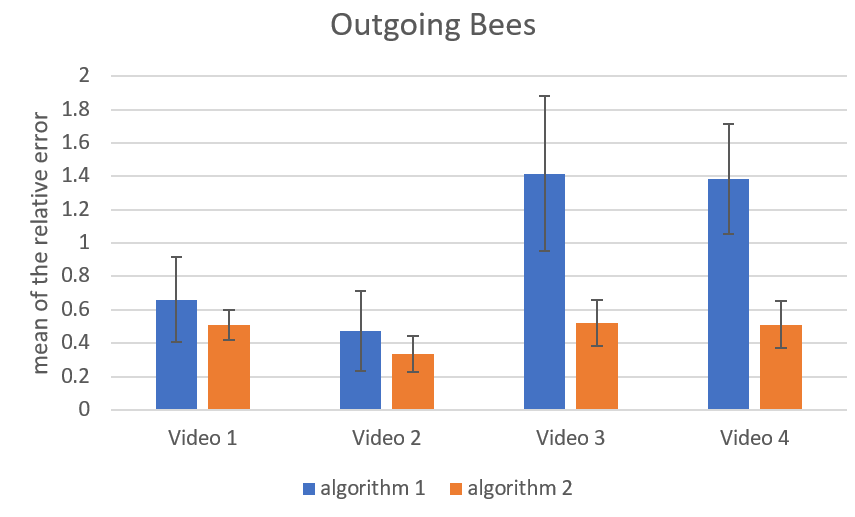
\includegraphics[width=\textwidth]{graphs/graph1.jpg}
        \caption{mean of relative error for the incoming flow of bees}
        \label{fig:meanRelative_1}
    \end{subfigure}
    \begin{subfigure}[b]{0.5\textwidth}
        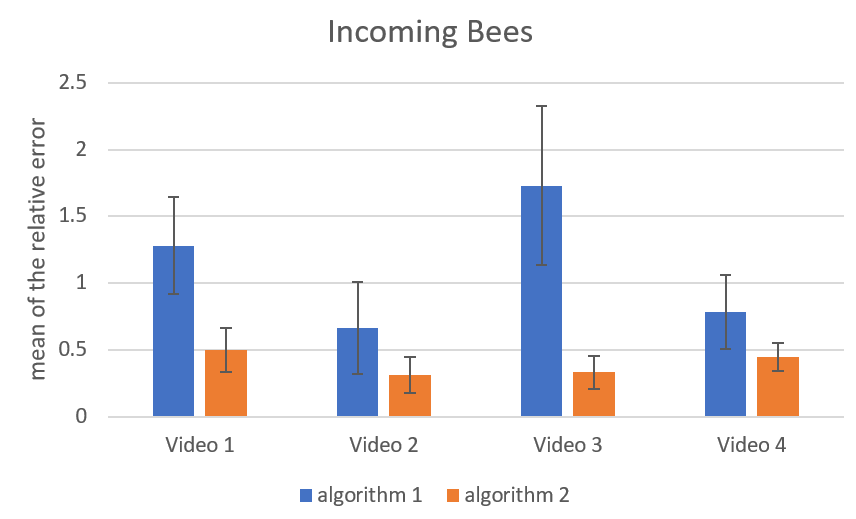
\includegraphics[width=\textwidth]{graphs/graph2.jpg}
        \caption{mean of relative error for the outgoing flow of bees}
        \label{fig:meanRelative_2}
    \end{subfigure}
\caption{Mean of relative errors with their respective standard error of the mean (SEM)}
\label{fig:meanRelative}
\end{figure}

An advantage of the first algorithm is that the algorithm is partially able to track the bees. As a consequence the algorithm is able to count bees whose detection failed while they were crossing the line. On the other hand, this leads to a major drawback of this algorithm. The problem occurs in the situation where several bees are sitting or moving close to the entry line. In that case the algorithm matches a lot of wrong bees. This depends a lot of the time we keep looking at a lost bee.\\
In general, errors mainly occur due to difficulties to detect bees if they are moving slowly. While most of the moving bees can be detected by our algorithm, we are still facing difficulties to distinguish overlapping bees. We have quite a large relative error, as stated, and we think it is mainly due to the difficulty of recognizing bees. E.g., in our implementation of tracking in algorithm 2, when we lose track of a bee in one frame only, we can’t retrieve this information and thus the tracking fails. Thus, the tracking performances are greatly dependent of the recognition performance. \\
The false recognition of other moving objects or shadows could be greatly reduced by our filters. While background subtraction was a good basis for our algorithm in the early stages, it turned out to be a limiting factor in terms of possibilities to reduce errors.

%------------------------------------------------------------------------
\section{Conclusion}

In this project, we implemented two algorithms able to detect and count the bees at the hive entrance. We got familiar with background subtraction as well as tracking methods in computer vision. We also got familiar with different functions from OpenCV.\\
For the future, the next steps would be to further improve bee recognition by other tools, such as machine learning, enhance the tracking algorithm and optimize the computational efficiency to use the program in real time.



{\small
\bibliographystyle{ieee}
\bibliography{egbib}
}

\end{document}